The experimental estimation for which out FFT becomes faster than the trivial DFT algorithm. 
\begin{center}
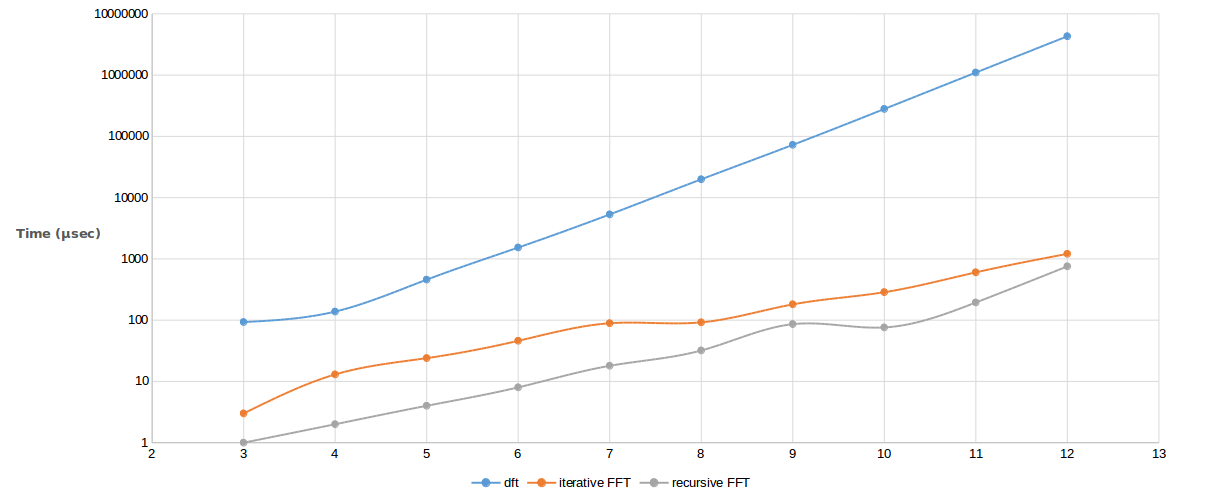
\includegraphics[width=\textwidth]{dft_comp.png}
\end{center}
Our FFT is faster from the beginning on.

Here is a comparison of Jupiter's and Saturn's performance of our iterative FFT. We did not include the recursive versions, since it is ways slower after \(2^{14}\) numbers.
\begin{center}
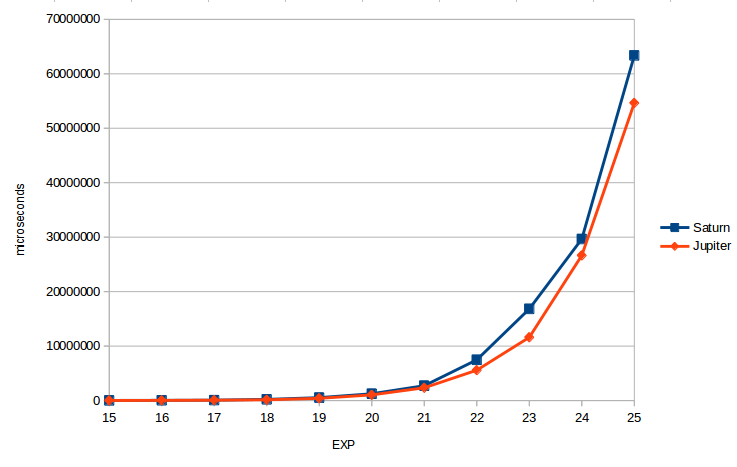
\includegraphics[width=\textwidth]{seq_performance.png}
\end{center}
Jupiter's of course faster. It got better CPUs. We used this information for our speedup plots later at our parallelism problem solutions.